\title{Proyecto con la Oficina de Responsabilidad Social Universitaria - PUJ, Cali.}
\author{Alejandro~Cardona,
        Luis~Santiago~Osorio,
        Diego~Lozada}

\date{\today}

\documentclass[12pt]{article}
\hoffset - 1cm % 2cm
\voffset - 0.54cm % 2cm
\setlength{\textwidth}{15.5cm}

\usepackage{dcolumn}
\usepackage{colortbl}
\usepackage{graphicx}
\usepackage{rotating}

\begin{document}
\maketitle
\tableofcontents
%% \begin{abstract}
%% This is the paper's abstract \ldots
%% \end{abstract}

\section{\textbf{Control de Versiones}}

\begin{tabular}{|>{\columncolor[gray]{0.7}} c |c|}
\hline
Vercion &\makebox[12.5cm][c]{1.0}\\
\hline
Fecha & 26/10/2012\\
\hline
Decripci\'on & Verci\'on inicial de documento de dise\~no\\
\hline
Autores & Alejandro Cardona\\
&Luis Santiago Osorio\\
&Diego Lozada\\
\hline
\end{tabular}

\section{Introduction}
\subsection{Proposito}
El siguente documento tiene como proposito especificar el diseño del proyecto con la oficina de responsabilidad social, mostrando la arquitectura, el manejo de datos y los subsistemas presentes.
\subsection{Alcance}
Se obtendr\'a una aplicaci\'on capas de gestionar \'e ingresar,
los proyectos relacionados con la oficina de responsabilidad social, y podra generar estad\'isticas a partir de los proyectos ingresados a el sistema.\\

El sistema dise\~nado podra realizar los siguentes procesos:

\begin{enumerate}
\item Agregar proyectos
\item Gestionar:
\begin{enumerate}
\item Crear.
\item Aceptar.
\item Clasificar.
\item Modificar.
\end{enumerate}
\item Generar estadisticas.
\item Generar Datos.
\end{enumerate}

\subsection{Objetivos}
El objetivo es lograr tener un diseño que cumpla con las caracteristicas basicas de un buen software, y que represente una buena erstructura que permita una buena mantenibilidad, robustes y seguridad.

\section{Tecnologia}
Para el desarrollo de la aplicaci\'on se utilizaran las diguentes herramientas:
\begin{itemize}
\item
Programas nesesarios:
\begin{itemize}
\item
\textbf{mysql 5.5.24} : MySQL es un sistema de gesti\'on de bases de datos relacional, multihilo y multiusuario. Es muy utilizado en aplicaciones web, como Drupal o phpBB, en plataformas (Linux/Windows-Apache-MySQL-PHP/Perl/Python), y por herramientas de seguimiento de errores como Bugzilla. Su popularidad como aplicaci\'on web est\'a muy ligada a PHP.\\
\item
\textbf{GlassFish} : GlassFish es un servidor de aplicaciones de software libre desarrollado por Sun Microsystems, compañía adquirida por Oracle Corporation, que implementa las tecnologías definidas en la plataforma Java EE y permite ejecutar aplicaciones que siguen esta especificación. \\
\end{itemize}
\item
Programas para la ncreaci\'on del programa:
\begin{itemize}
\item
\textbf{JDK 7} : Java Development Kit o (JDK), es un software que provee herramientas de desarrollo para la creaci\'on de programas en Java.\\
\item
\textbf{NetBeans IDE 6 o 7} : NetBeans es un entorno de desarrollo integrado libre, hecho principalmente para el lenguaje de programaci\'on Java. Existe adem\'as un n\'umero importante de m\'odulos para extenderlo.\\
\end{itemize}
\end{itemize}

\section{Arquitectura del sistema}
La arquitectura de el sistema se realizara en un modelo por capas, en este modelo estan los siguentes modulos:\\

\subsection{Usuarios} 
Son las personas involucradas en el manejo del sistema.
\subsection{Interfaz de usuario}
En esta capa se contendr\'a la interfaz gráfica de usuario en la que podra interactuar con el sistema.
\subsection{Componentes de logica}
Esta capa contendra la lógica y reglas para almacenar datos en la capa que accede a la base de datos dando restricciones segun el usuario que ingrese y a su ves, tambi\'en para recuperar éstos de acuerdo con las necesidades y restricciones del usuario.
\subsection{Componentes de acceso a la Base de datos}
Esta capa manejara las consultas y commits a la base de datos, segun los llamados que genere la capa logica.
\subsection{Origenes de datos}
En esta capa se encontraran almacenados los datos del sistema.
\subsection{Seguridad}
Controlara la seguridad del sistema, manejando el cifrado de claves y de mas.
\subsection{Diagrama de arquitectura por capas}
\begin{center}
\rotatebox{0}{\scalebox{1}[1]{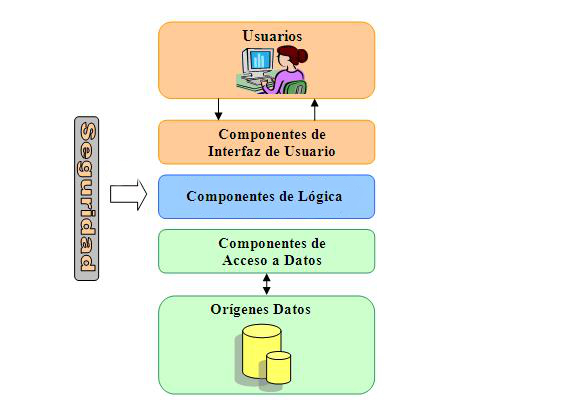
\includegraphics[width=10cm,height=8cm]{arquitectura.jpg}}}
\end{center}

%% \begin{tabbing}
%% \hspace*{1cm} 
%% \end{tabbing}
%% \begin{tabbing}
%% \hspace*{1cm} 
%% \end{tabbing}
%% \begin{tabbing}
%% \hspace*{1cm} 
%% \end{tabbing}
%% \begin{tabbing}
%% \hspace*{1cm} 
%% \end{tabbing}
%% \begin{tabbing}
%% \hspace*{1cm} 
%% \end{tabbing}



\section{Diagrama de clases del sistema}
En este diagrama se describe la estructura del sistema mostrando sus clases, atributos y las relaciones entre ellos, y se vera la informaci\'on que se manejar\'a en el sistema, y los componentes que se encargaran del funcionamiento y la relaci\'on entre uno y otro.
Se agrega imagen completa para mejor visualisaci\'on

\begin{center}
\rotatebox{0}{\scalebox{1}[1]{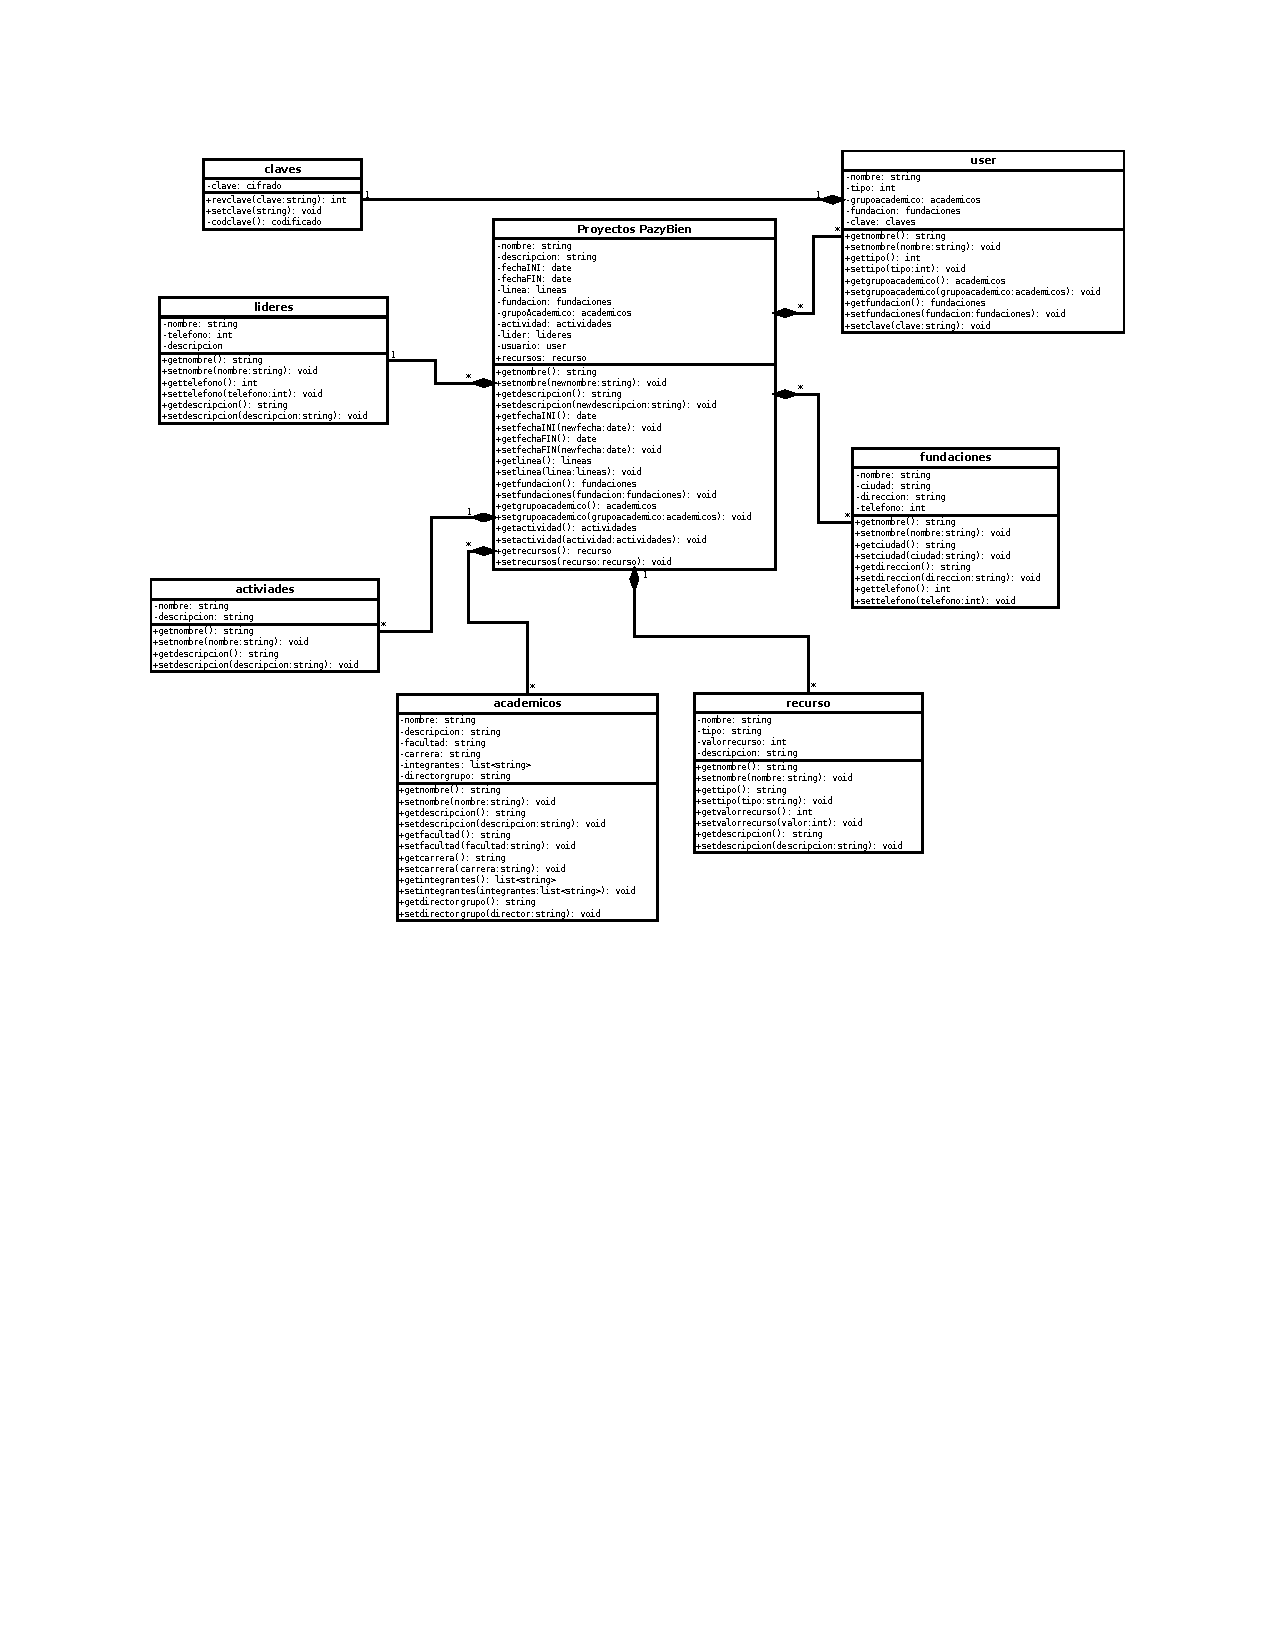
\includegraphics[width=16cm,height=22cm]{diagramaclases.pdf}}}
\end{center}

\section{Diagramas de secuencia}

\bibliographystyle{abbrv}
\bibliography{main}

\end{document}
This is never printed
